\documentclass[10pt,conference,compsocconf]{IEEEtran}

\usepackage{hyperref}
\usepackage{graphicx}
\usepackage{xcolor}
\usepackage{blindtext, amsmath, comment, epsfig }
\usepackage{caption}
\usepackage{subcaption} % or subfig
\usepackage{cleveref} % cref
\usepackage{amsfonts} 
\usepackage{algorithmic}
\usepackage{cite}
\usepackage[utf8]{inputenc}


\IEEEaftertitletext{\vspace{-1\baselineskip}}

\usepackage{scalerel}
\DeclareMathOperator*{\concat}{\scalerel*{||}{\sum}}


\usepackage{listings}
\usepackage{color}
\definecolor{dkgreen}{rgb}{0,0.6,0}
\definecolor{gray}{rgb}{0.5,0.5,0.5}
\definecolor{mauve}{rgb}{0.58,0,0.82}
\lstset{language=SQL,
  basicstyle={\small\ttfamily},
  belowskip=3mm,
  breakatwhitespace=true,
  breaklines=true,
  classoffset=0,
  columns=flexible,
  commentstyle=\color{dkgreen},
  framexleftmargin=0.25em,
  frameshape={}{yy}{}{}, %To remove to vertical lines on left, set `frameshape={}{}{}{}`
  keywordstyle=\color{blue},
  numbers=none, %If you want line numbers, set `numbers=left`
  numberstyle=\tiny\color{gray},
  showstringspaces=false,
  stringstyle=\color{mauve},
  tabsize=3,
  xleftmargin =1em
}

\title{\Large GeoPKI \vspace{-1.1em}}
% \author{}
\date{}



\ifdefined\final
\newcommand{\todo}[1]{}
\newcommand{\ck}[1]{}
\newcommand{\ckrm}[1]{}
\newcommand{\chrissy}[1]{}
\else
\newcommand{\todo}[1]{\textcolor{red}{\emph{\textbf{[TODO: }#1\textbf{]}}}}
\newcommand{\ck}[1]{\textcolor{violet}{\emph{\textbf{cyrill: }#1}}}
\newcommand{\ckrm}[1]{\textcolor{violet}{\emph{\textbf{cyrill remove:} ``#1''}}}
\newcommand{\chrissy}[1]{\textcolor{blue}{\emph{\textbf{chrissy: }#1}}}
\newcommand{\nico}[1]{\textcolor{orange}{\emph{\textbf{nico: }#1}}}
\fi

\begin{document}

\makeatletter
\@twocolumnfalse
\maketitle
\@twocolumntrue
\makeatother

%\begin{abstract}
%\end{abstract}


% \section{Introduction}
% \label{introduction}

\section{Model}
\label{sec:model}

The earth ellipsoid model of the existing world geodetic system 84 (WGS84) \cite{noauthor_nga_nodate} is used.
WGS84 defines the \emph{semi-major axis} (half of the largest diameter of an ellipsoid, at the equator) $a$ to be $6'378'137.0$~meters \cite{noauthor_nga_nodate}. The \emph{semi-minor axis} (the polar radius) $b$ is defined as $6'356'752.3142~$meters \cite{noauthor_nga_nodate}.
Standard polar coordinates (longitude, latitude) are used for referencing points on the planet's two-dimensional surface and a third coordinate, altitude, extends this to three dimensions.
Longitude, latitude and altitude together refer to a unique point in three-dimensions.

Each of the three coordinates is discretized in a way that preserves $u := 1$ meter-precision in the worst case.
With the semi-major axis $a$, the maximum circumference of the ellipsoid equals $=2 a \pi$~meters.
Using base two, $B_{x}:= \left\lceil \log_2(\frac{2 a \pi}{u}) \right\rceil = 26$ bits for the longitude thus suffice to represent each possible meter value in the worst case.
Let $C_{x} := 2^{B_{x}} - 1$ denote the maximum discretized value for the longitude.
For the latitude the circumference is $2 b \pi$~meters but we only need to be able to represent half of it, so $b \pi$.
Thus $\left\lceil\log_2(\frac{b \pi}{u})\right\rceil = 25 =: B_{y}$ bits suffice.
Analogously to $C_{x}$, let $C_y := 2^{B_{y}} - 1$ the maximum discretized value for the latitude.
For altitude there is no natural bound so one has to be fixed.
At the time of writing, the highest point on earth is below $10'000$~meters above sea level \cite{us_department_of_commerce_what_nodate} and the lowest layer of earth's atmosphere, the troposphere, extends to about $18$~km \cite{dhaka_chapter_2023}.
The Mariana Trench at about $10'000$~m below sea level \cite{gardner_so_2014} is likely a bound not exceeded in the near future.
The necessity of allowing volumes below sea level arises from countries such as the Netherlands where parts of the surface's altitude is below sea level \cite{kabat_climate_2005} .
Moreover in the future, below sea level research stations might be built.
Thus the range starting at a depth of $D:=-10'000$~m up to an altitude of $20'000$~m above sea level should cover any current and near-future needs.
Covering this range requires $B_{z} := \left\lceil \log_2(\frac{H - D}{u}) \right\rceil = 15$ bits.
In fact using $B_z$ bits starting at $D$ will cover the range from $D$ to $D + (2^{B_{z}} - 1) \cdot u = 22'767 := H$.
Complications might arise from distance calculations when using sea level as a reference as the sea level is not the same in all places and will increase in the future.
Thus instead of using sea level as a reference, the geodetic altitude defined by WGS84~\cite{noauthor_nga_nodate} is used.
Given the geoid's surface in WGS84 is about at the mean sea level (MSL), the range $[D, H]$ can be left as is.
While it does not exactly cover the range described range with respect to local sea level, it approximates it.

\section{Data Structure}
\label{sec:data-structure}

Inspired by F-PKI~\cite{chuat_f-pki_2022}, a sparse merkle hash tree (SMT) is used.
Each leaf represents a full discretized coordinate using $B := \cdot B_{x} + B_{y} + B_{z} = 66$ bits resulting in a total of $2^{B}$ leaves.
To have spatially close points somewhat close together in the SMT, the space-filling $Z$-order curve is used to sort the three dimensional locations in one dimension \cite{morton_computer_1966}.
An example with $B_{x} = B{y} = B_{z} = 2$ is shown in \Cref{fig:z-curve-example:two-bits}.
GeoPKI uses a slightly modified 3D Z-order curve:
Rather than using the full 3D Z-order curve, a 2D Z-order curve over the longitude and latitude is used and points with the same longitude and latitude but different altitude are put in sequence.
While this leads to spatially close points being further apart in the 1-dimensional sorting, this modification allows for shorter proofs under some assumptions (will be discussed in \Cref{sec:optimizations}).
\Cref{fig:z-curve-example:two-bits-optim} contrasts this modification with the standard 3D Z-order curve shown in \Cref{fig:z-curve-example:two-bits}.

\subsection{Leaf Binary Format}
\label{sec:data-structure:leaf-binary}
Each leaf of the SMT corresponds to a point and the tree leaves are sorted lexicographically by their binary representation in ascending order.
A point tuple $p := (x,y,z)$ at longitude $x$, latitude $y$ and altitude $z$ with
\begin{align*}
	(x, y, z) &\in [-180, 180] \times [-90, 90] \times [D, H]
\end{align*}

is first discretized to integer coordinates as follows:

\begin{align}
\begin{split}
\label{eq:discretization}
p' :&=
(x_d,y_d, z_d)
\\
& =
\left(
%
\left\lfloor
\frac{x + 180}{360} \cdot C_x
\right\rfloor,
%
\left\lfloor
\frac{y + 90}{180} \cdot C_y
\right\rfloor,
%
\left\lfloor
\frac{z - D}{u}
\right\rfloor
%
\right)
\end{split}
\end{align}

After this transformation the following folds:

\begin{align*}
	p' &\in [0, 2^{B_x}) \times [0, 2^{B_y}) \times [0, 2^{B_z})
\end{align*}

This formula holds since the first term in the longitude and latitude tuples can be at most $1$ and since $C_x$ and $C_y$ are the maximum values that can be represented using $B_x$ and $B_y$ bits, respectively.
Moreover $H - D = 2^{B_z} - 1$ holds meaning the altitude can be represented using $B_z$ bits.
The three resulting integer numbers can now be represented using $B_{x}$, $B_{y}$ and $B_z$ bits, respectively. Let $p'' := (x_b, y_b, z_b)$ be their big-endian integer binary encoding with
\begin{align*}
	p'' &\in \{0,1\}^{B_{x}} \times \{0,1\}^{B_{y}} \times \{0,1\}^{B_z}
\end{align*}

For $c \in \{x, y, z\}$ and for any integer $i \in \{0, ..., B_c-1\}$, let $c_{b,i}$ denote the $i$-th bit of $c_{b}$. Moreover let $||$ denote the concatenation operator.
The binary representation $p_b$ of the point $p$ is then defined as
\begin{align*}
	p_b = \left(\concat_{i=0}^{B_{y} - 1} x_{b,i} || y_{b,i} \right) || x_{b,B_{x}-1} || \left(\concat_{i=0}^{B_{z}-1} z_{b,i} \right)
\end{align*}

In words, the binary representation of $p$ is the interleaving of the binary representation for the longitude and latitude concatenated to the binary representation of the altitude.

\Cref{fig:leaf-representation:binary} shows an example of this binary encoding.

% ($47.37643$, $8.54828$, $0$)

%Storing a dense SMT with $2^{B} \leq (2^{10})^7 \approx (10^3)^7 = 10^{21}$ leaves is certainly infeasible but under the assumption that most leaves are empty it seems reasonable.

\begin{figure}
    \centering
    \begin{subfigure}[t]{0.24\textwidth}
        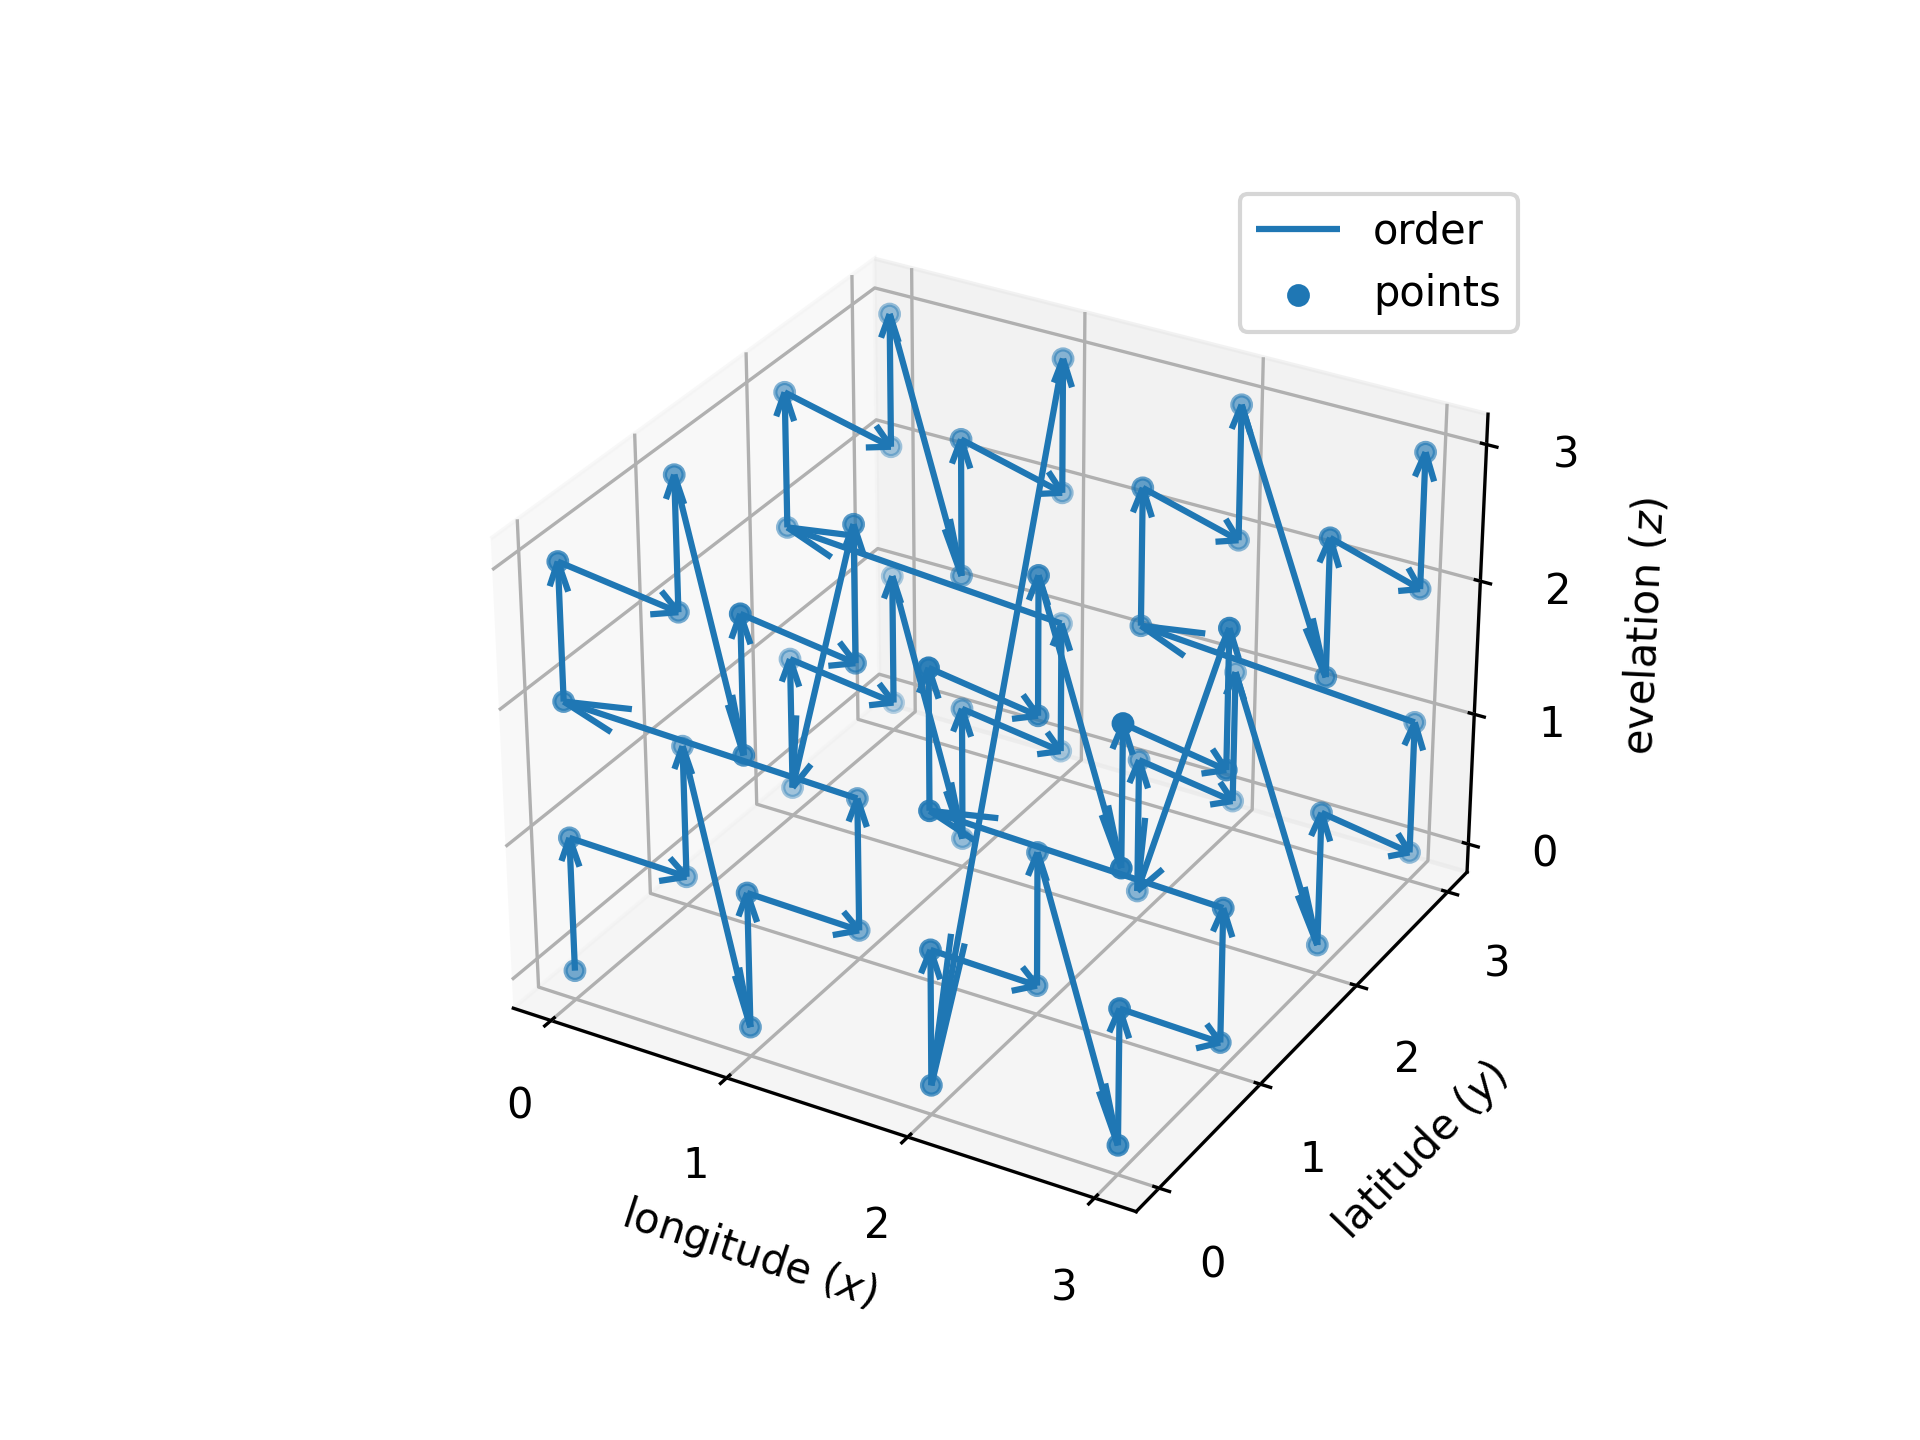
\includegraphics[width=\textwidth]{./resources/z-example/two-bits-z.png}
        \caption{3D Z-Order Curve}
        \label{fig:z-curve-example:two-bits}
    \end{subfigure}
    \hfill
    \begin{subfigure}[t]{0.24\textwidth}
        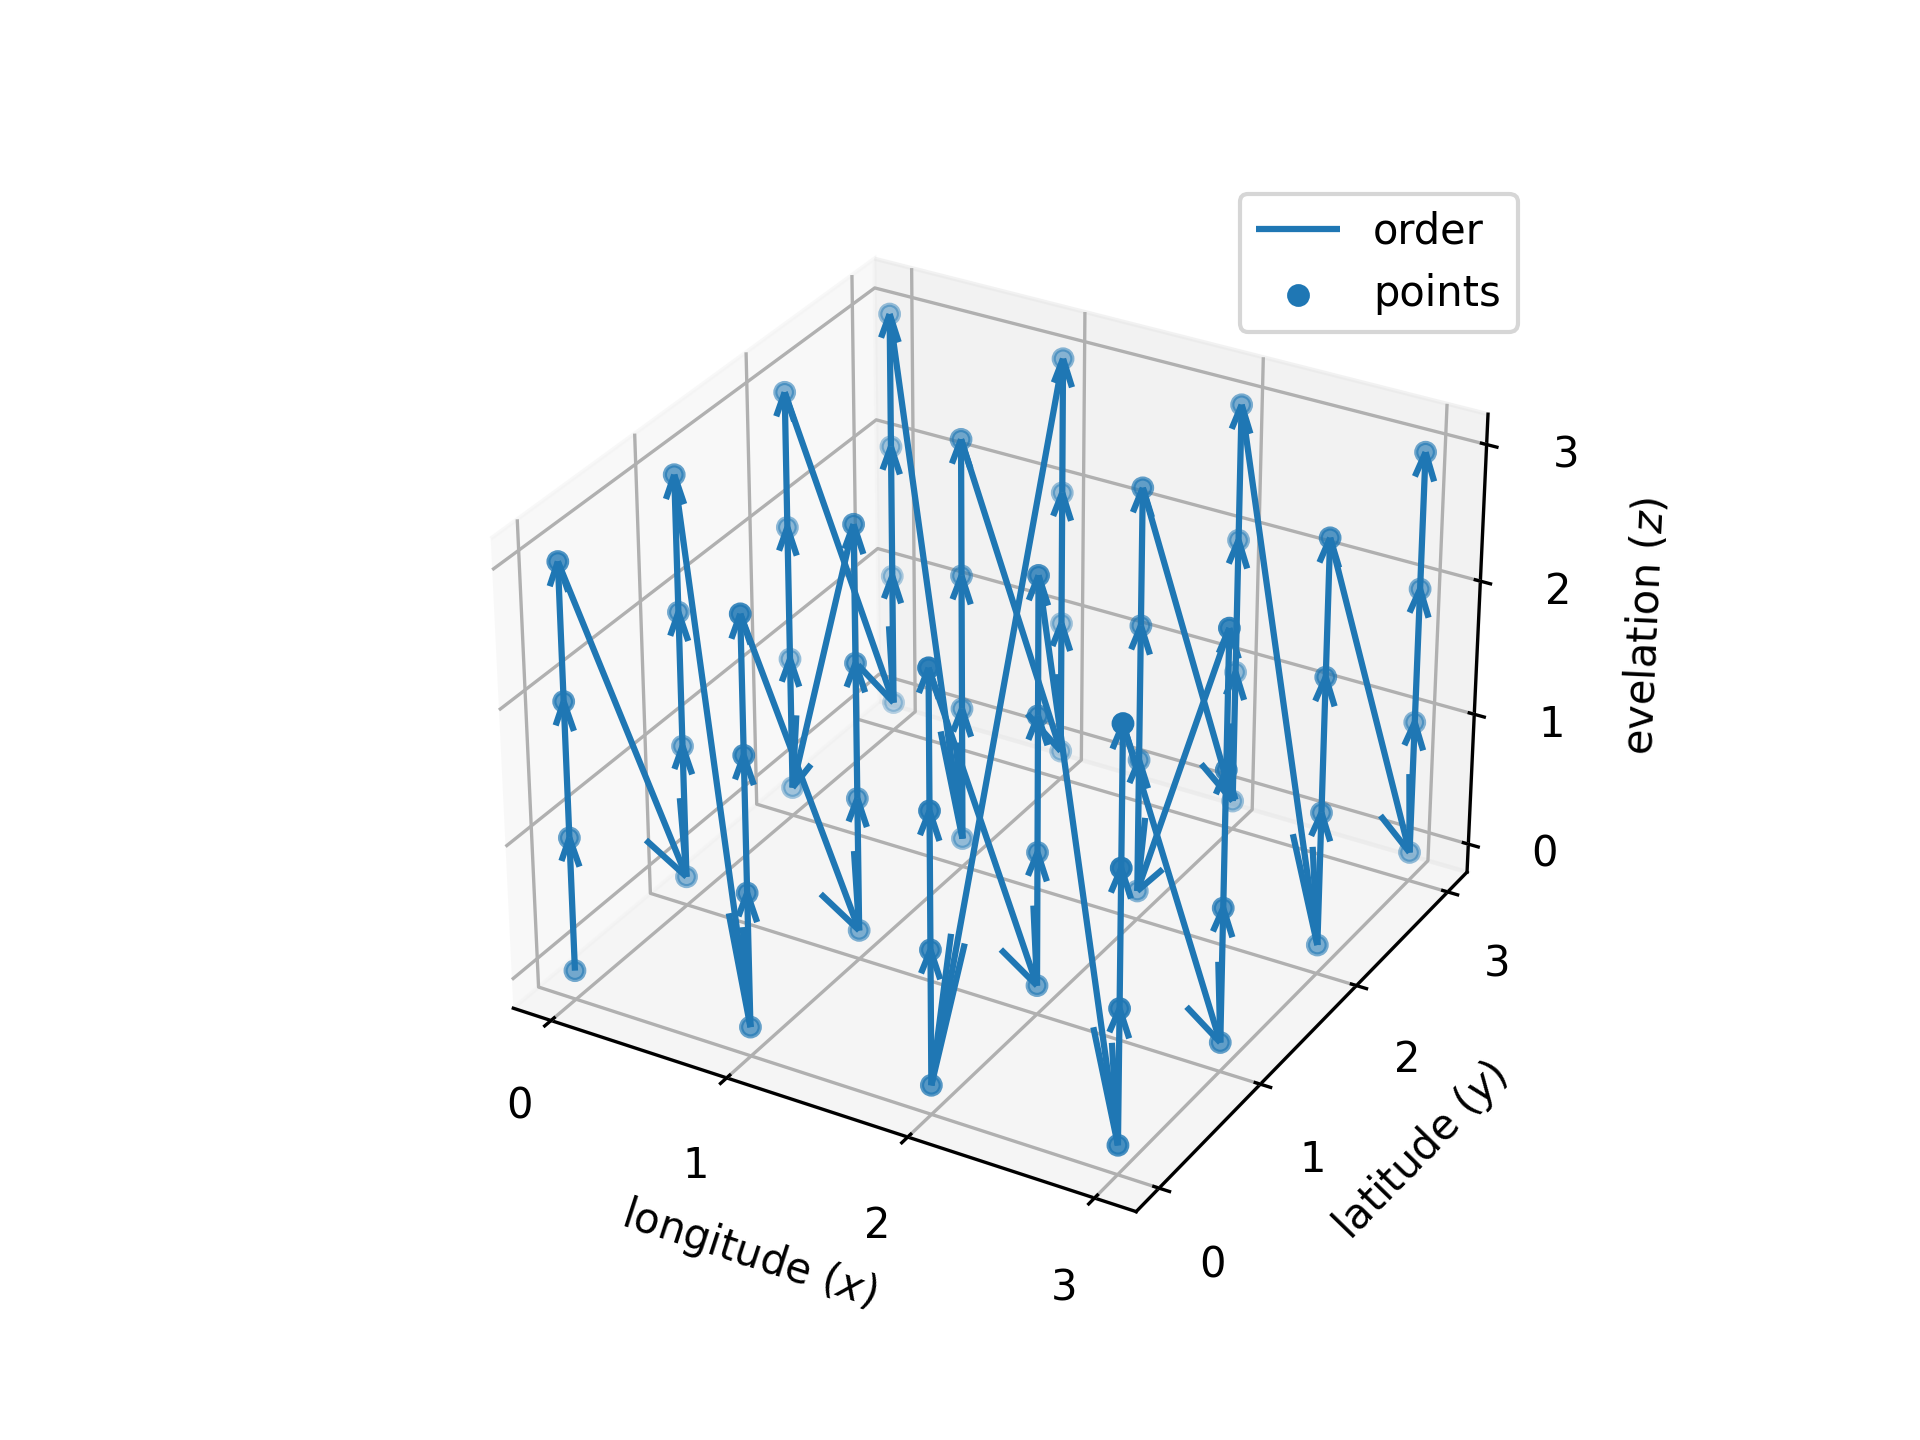
\includegraphics[width=\textwidth]{./resources/z-example/two-bits.png}
        \caption{2D Z-Order Curve with altitude in sequence}
        \label{fig:z-curve-example:two-bits-optim}
    \end{subfigure}
    \caption{
    	Difference between a standard 3D Z-order curve and the one used by GeoPKI when using two bits for all coordinates.
    }
    \label{fig:z-curve-example}
\end{figure}

\subsection{Leaf Geometric Representation}
\label{sec:data-structure:leaf-geometry}
Due to the floor functions in \Cref{eq:discretization}, the point $p''$ represents the volume where $p''$ is in the corner with the smallest coordinates in all three dimensions.
By replacing the floor functions by mathematically rounding or the ceil function the volumetric representation changes.
In case of the floor functions shown in \Cref{eq:discretization}, the point corresponding to $p''$ is
\begin{align}
\begin{split}
\label{eq:leaf-geometric-point}
\left(x_d \cdot \frac{360}{C_x} - 180,x_d \cdot \frac{180}{C_y} - 90, z_d \cdot u + D\right)
\end{split}
\end{align}
and the volume represented by point $p''$ is given by
\begin{align}
\begin{split}
\label{eq:leaf-geometric-volume}
\left[x_d \cdot \frac{360}{C_x} - 180, (x_d + 1) \cdot \frac{360}{C_x} - 180\right) &\times\\
\left[y_d \cdot \frac{180}{C_y} - 90, (y_d + 1) \cdot \frac{180}{C_y} - 90\right) &\times\\
\left[D + z_d \cdot u, D + z_d \cdot u + 1 \right)&
\end{split}
\end{align}

\Cref{fig:leaf-representation:geometric} shows the points and the corresponding volumes in the same color.

\begin{figure}
    \centering
    \begin{subfigure}[t]{0.24\textwidth}
        
\includegraphics[width=\textwidth]{./resources/leaf-representation/binary-representation.pdf}
        \caption{Binary Representation of a (longitude, latitude, altitude) tuple.}
        \label{fig:leaf-representation:binary}
    \end{subfigure}
    \hfill
    \begin{subfigure}[t]{0.24\textwidth}
        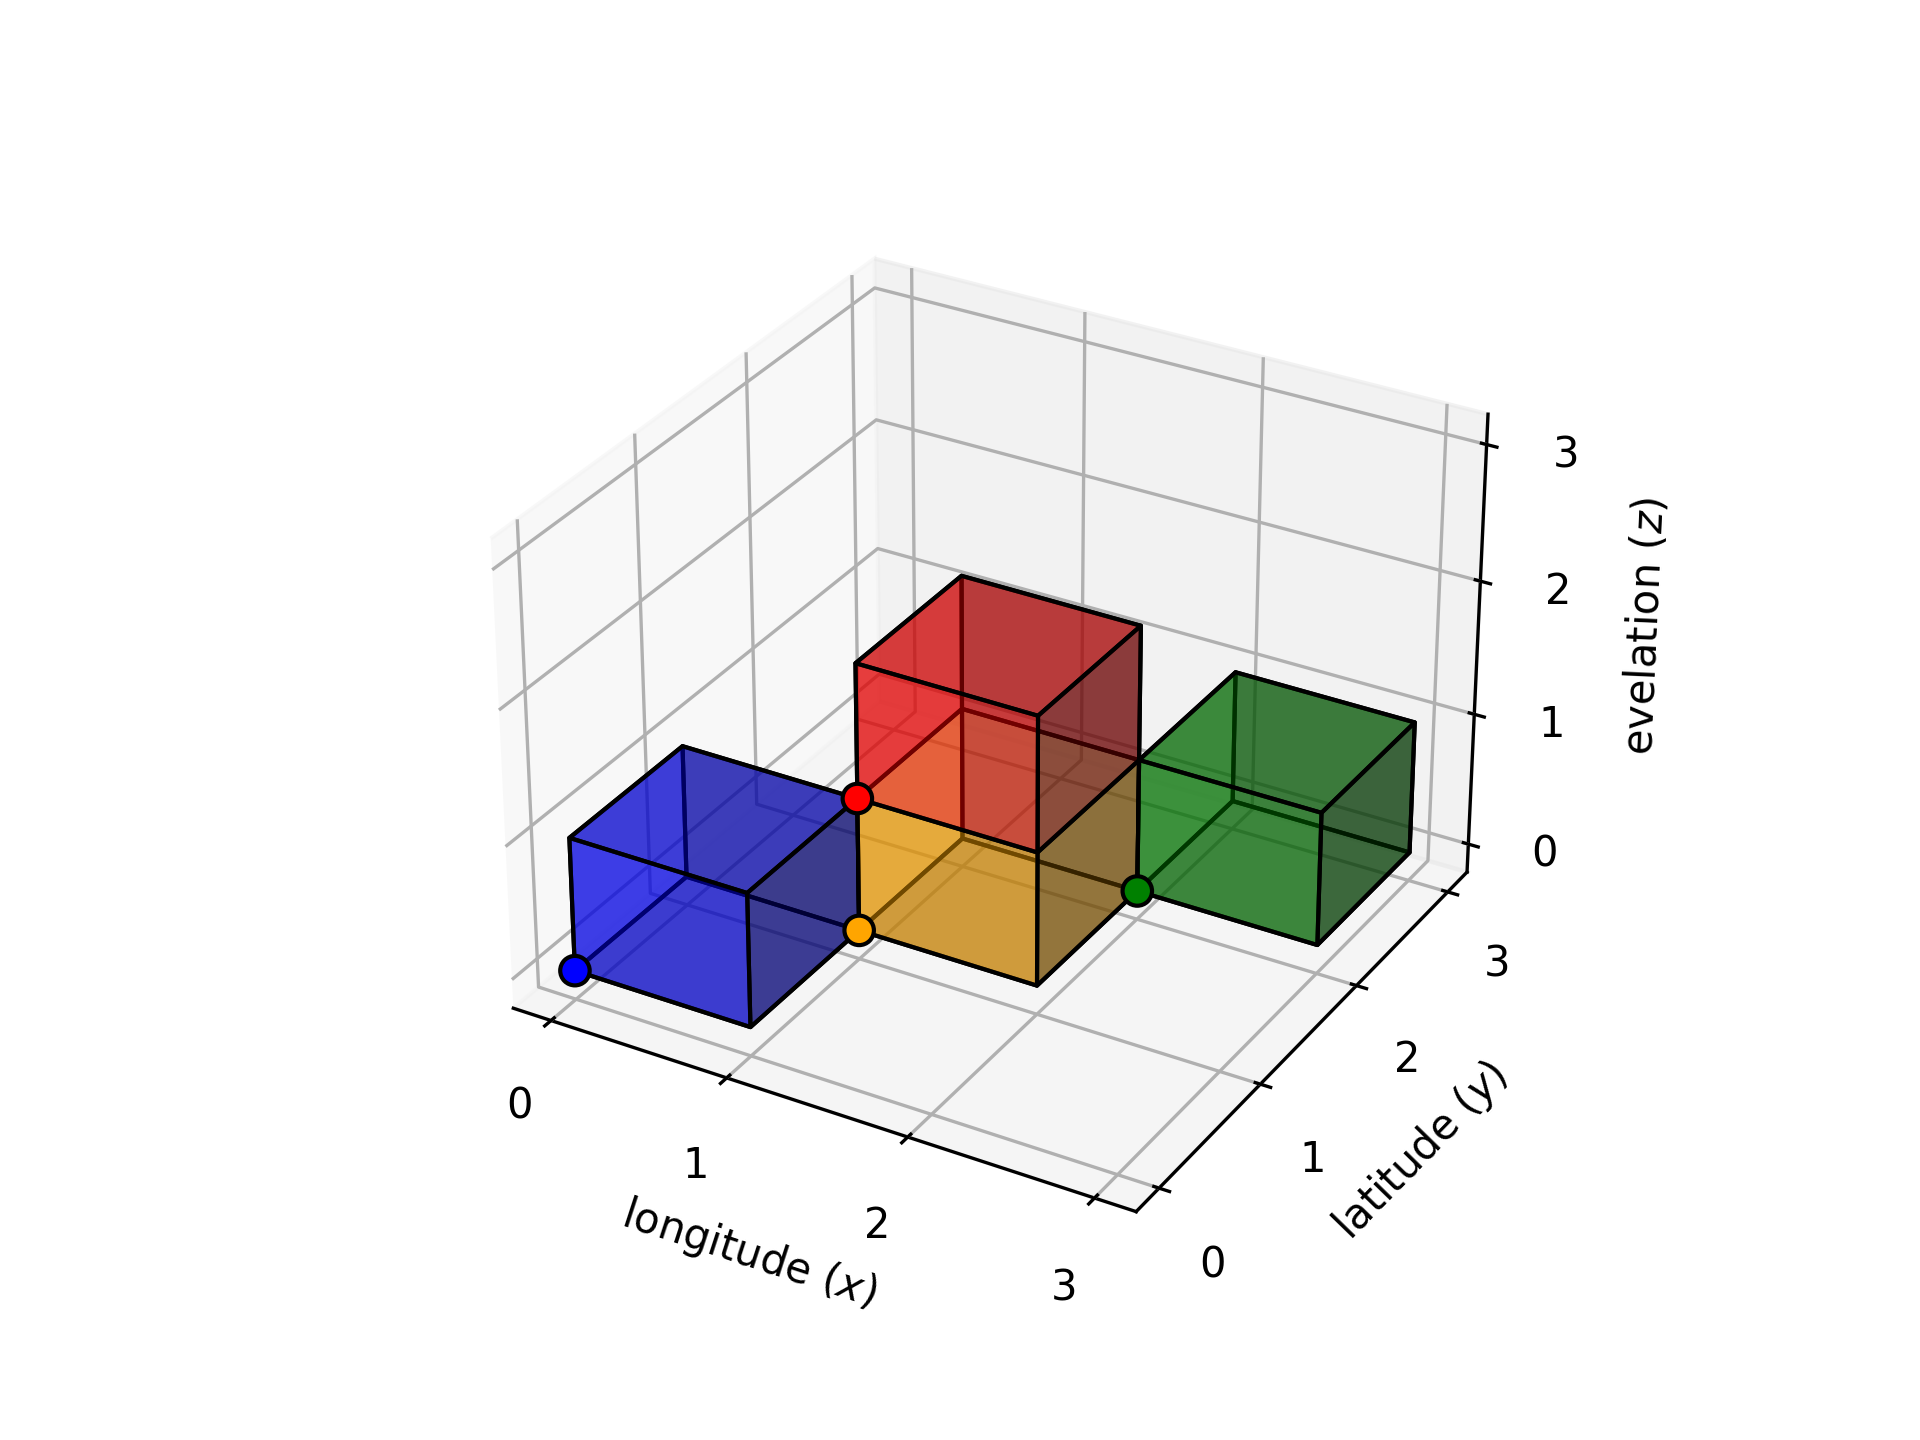
\includegraphics[width=\textwidth]{./resources/leaf-representation/geometric-representation.png}
        \caption{Geometric Representation}
        \label{fig:leaf-representation:geometric}
    \end{subfigure}
    \caption{
    	The binary and geometric representation of a leaf
    }
    \label{fig:leaf-representation}
\end{figure}

\subsection{Intermediate Nodes}
\label{sec:data-structure:intermediate}
Intermediate nodes in the SMT also correspond to a point and a volume following the same pattern as for the leaf nodes.
The bit string corresponding to an intermediate node is simply the longest common prefix of it's two children and covers the whole volume of its two children.
The left child is the node with the binary representation equal to the intermediate node one's concatenated with a zero and the right child concatenated with a one.
The formula for computing the volume becomes more complex for intermediate nodes as it requires a case distinction:
Let $s$ be the bit string of an intermediate node.

Let $l$ be the length of $s$.
Let $s_x$, $s_y$, $s_z$ be the bit prefixes encoded in $s$ corresponding to the longitude, latitude and altitude, respectively.
Moreover let $l_x$, $l_y$ and $l_z$ be the lengths of $s_x$, $s_y$ and $s_z$, respectively, and let $s_{c,i}$ for $i \in \{0, ..., l_c-1\}$ and $c \in \{x, y, z\}$ correspond to the $i$-th bit of $s_c$.
It holds that $l = l_x + l_y + l_z$ and it is possible that $l_x$ is by exactly one larger than $l_y$, otherwise $l_x = l_y$.
This directly follows from the interleaved binary encoding described in \Cref{sec:data-structure:leaf-binary}.
Let $x'_d$, $y'_d$, $z'_d$ be the most-precise integers that can be re-constructed with the given bits:
\begin{align}
	\label{eq:intermediate-geometric-point-partial-height:x}
	x'_d :&= \sum_{i=0}^{l_x - 1} 2^{B_{x,y} - 1 - i} \cdot s_{x,i}\\
	\label{eq:intermediate-geometric-point-partial-height:y}
	y'_d :&= \sum_{i=0}^{l_y - 1} 2^{B_{x,y} - 1 - i} \cdot s_{y,i}\\
	\label{eq:intermediate-geometric-point-partial-height:z}
	z'_d :&= \sum_{i=0}^{l_z - 1} 2^{B_{z} - 1 - i} \cdot s_{z,i}
\end{align}

Then the corresponding point is given by
\begin{align}
\begin{split}
\label{eq:intermediate-geometric-point-partial-height}
\left(x'_d \cdot \frac{360}{C_x} - 180,y_d \cdot \frac{180}{C_y} - 90, D + z'_d \cdot u\right)
\end{split}
\end{align}
and the covered volume by
\begin{align}
\begin{split}
\label{eq:intermediate-geometric-volume-full-height}
\left[x'_d \cdot \frac{360}{C_x} - 180, (x_d + 2^{B_{x,y} - l_x}) \cdot \frac{360}{C_x} - 180\right) &\times\\
\left[y'_d \cdot \frac{180}{C_y} - 90, (y_d + 2^{B_{x,y} - l_y}) \cdot \frac{180}{C_y} - 90\right) &\times\\
\left[D + z'_d \cdot u, D + \left(z'_d + 2^{B_z - l_z}\right) \cdot u\right)&
\end{split}
\end{align}

This is the more general form of \Cref{eq:leaf-geometric-volume} and for $l_x = l_y = B_{x,y}$ and $l_z = B_z$ the two are equivalent.

It is worth nothing is that in GeoPKI, intermediate nodes also store a set of certificates.
When using a tree representing the geography (which can reduce proof sizes as described in \Cref{sec:alternative-designs}), this is almost a requirement.
Without this optimization, almost no leaf would be empty as almost all pieces of land on earth are claimed by at least one country.
This would require enormous storage costs and result in less efficient queries.

\subsection{Sparse Merkle Hash Tree (SMT)}
\label{sec:data-structure:SMT}

The just described tree is combined with a SMT.
As in F-PKI \cite{chuat_f-pki_2022}, each leaf stores a set of certificates.
Let $C_0, C_1, ..., C_{n-1}$ be the sequence of certificates located in a leaf, sorted lexicographically by their SHA-256 hashes in ascending order.
The hashes are computed on the PEM encoding of the X.509 certificates.
The leaf's hash value is then defined as
\begin{align}
	\label{eq:hash-leaf}
	H(0 || H(C_0) || H(C_1) || ... || H(C_n))
\end{align}
where $H$ is SHA-256.
The hash value of an empty / non-existent leaf or intermediate node in the SMT is $H(0)$.
An intermediate node in the tree has two children (two intermediate nodes or two leaves) and in GeoPKI also stores a set of certificates.
As before, let $C_0, C_1, ..., C_{n-1}$ be the sequence of certificates located in an intermediate node, sorted lexicographically by the SHA-256 hashes of the PEM encoding in ascending order.
Hash $h_3$ over the list of certificates is defined as
\begin{align}
	\label{eq:hash-certs-intermediate-node}
	h_3 := H(H(C_0) || H(C_1) || ... || H(C_n))
\end{align}

Then let $h_1$ and $h_2$ be the hash values of the left and right child of the intermediate node, respectively.
The hash value of the intermediate node is then defined as

\begin{align}
	\label{eq:hash-intermediate-node}
	\left\{
	\begin{array}{lr}
		H(1 || h_1 || h_2) & \text{if $n = 0$}\\
		H(1 || h_1 || h_2 || h_3) & \text{if $n > 0$}
	\end{array}\right.
\end{align}

The constants $0$ and $1$ are prefixed in the hash computation to prevent collisions where a given hash $H(a || b)$ for some $a$ and $b$ could simultaneously refer to a leaf with content $a || b$ or a intermediate node with children hash values $a$ and $b$.

%\subsection{Querying the SMT}
%\label{sec:data-structure:query}
%
%Since many sizes of volumes can be represented by the binary format described in Sections \ref{sec:data-structure:leaf-binary} and \ref{sec:data-structure:intermediate}, it is for now assumed that the only type of query a GeoPKI map server supports is such a bit string.
%Such a bit string has a unique corresponding node in the tree (that might not exist as the tree is sparse).
%The result then is the set of all certificates stored at intermediate nodes above the specified node (as these represent larger areas covering the queries point) and the set of all certificates stored in the subtree rooted at the specified node as these are within the queried area.
%The former set corresponds to the set of nodes whose corresponding binary representation are a prefix for the given query.
%The latter set corresponds to the set of nodes whose corresponding binary representation the given query is a prefix for.
%
%A trivial way to obtain this set of certificates is to walk the tree from the root and collect the certificates stored at the intermediate nodes along the way.
%If the next bit is a zero, go left, if it is one, go right.
%Once the node with a bit string corresponding to the query is found, the full subtree rooted at this node is walked recursively until an empty node or a leaf is found and all found certificates are returned.

\subsection{Arbitrary Volumes and Certificate Placement}
\label{sec:data-structure:arbitrary-volumes}

\begin{figure}
    \centering
    \begin{subfigure}[t]{0.11\textwidth}
        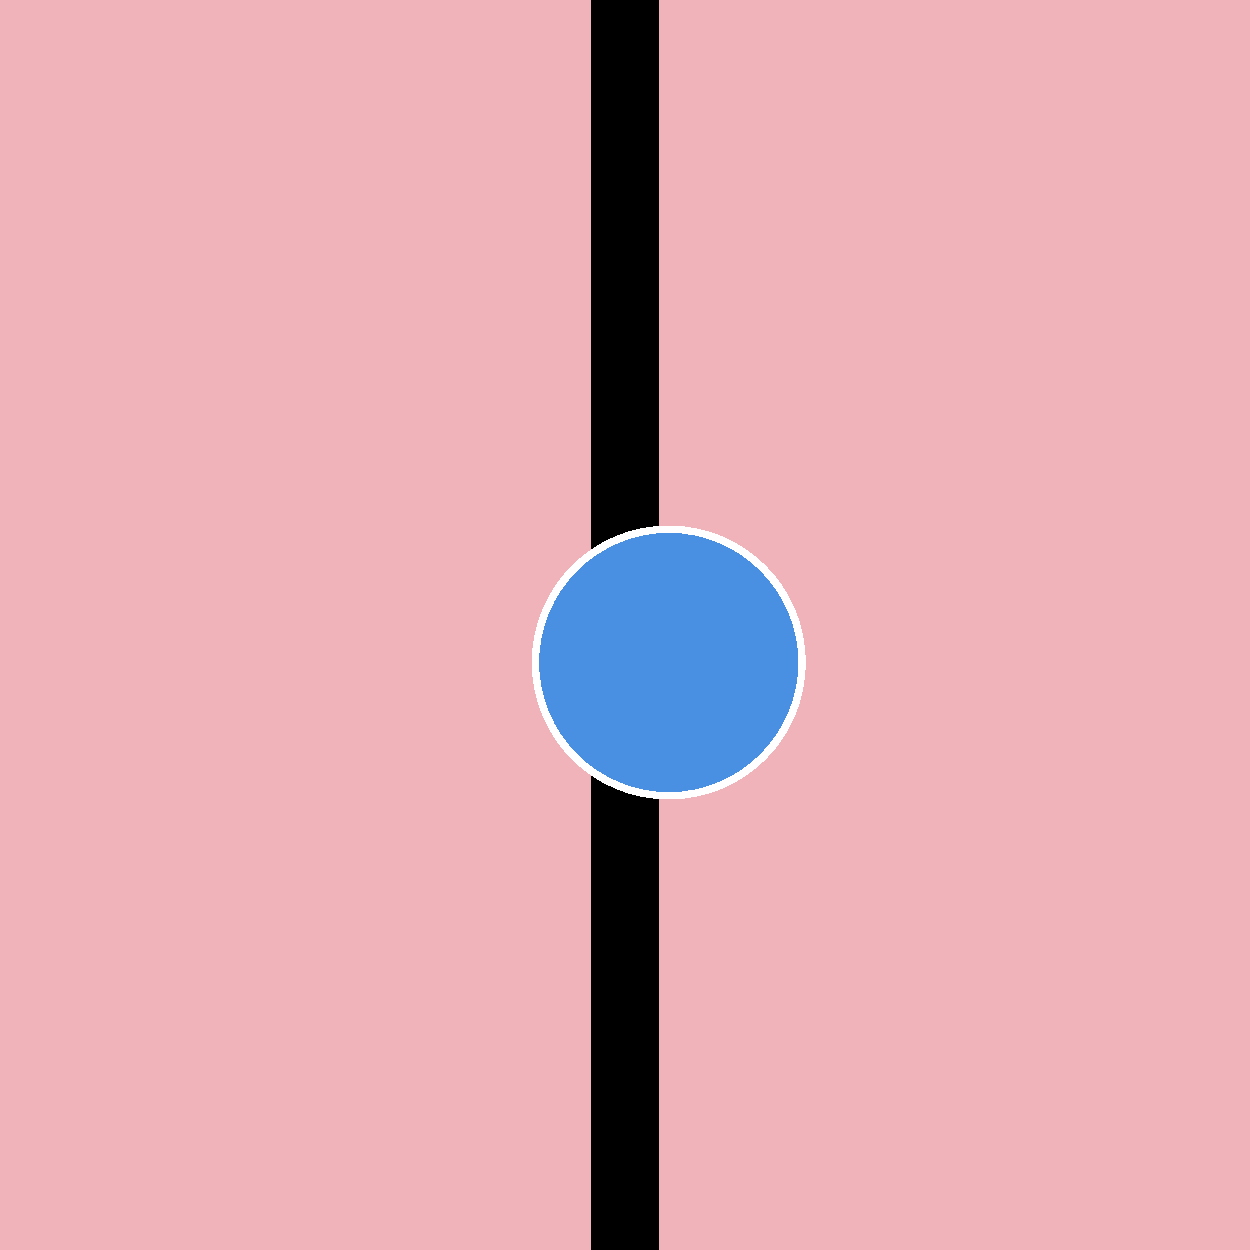
\includegraphics[width=\textwidth]{./resources/worst-case/worst-case-1.pdf}
        \caption{Areas after one split}
        \label{fig:worst-case:one}
    \end{subfigure}
    \hfill
    \begin{subfigure}[t]{0.11\textwidth}
        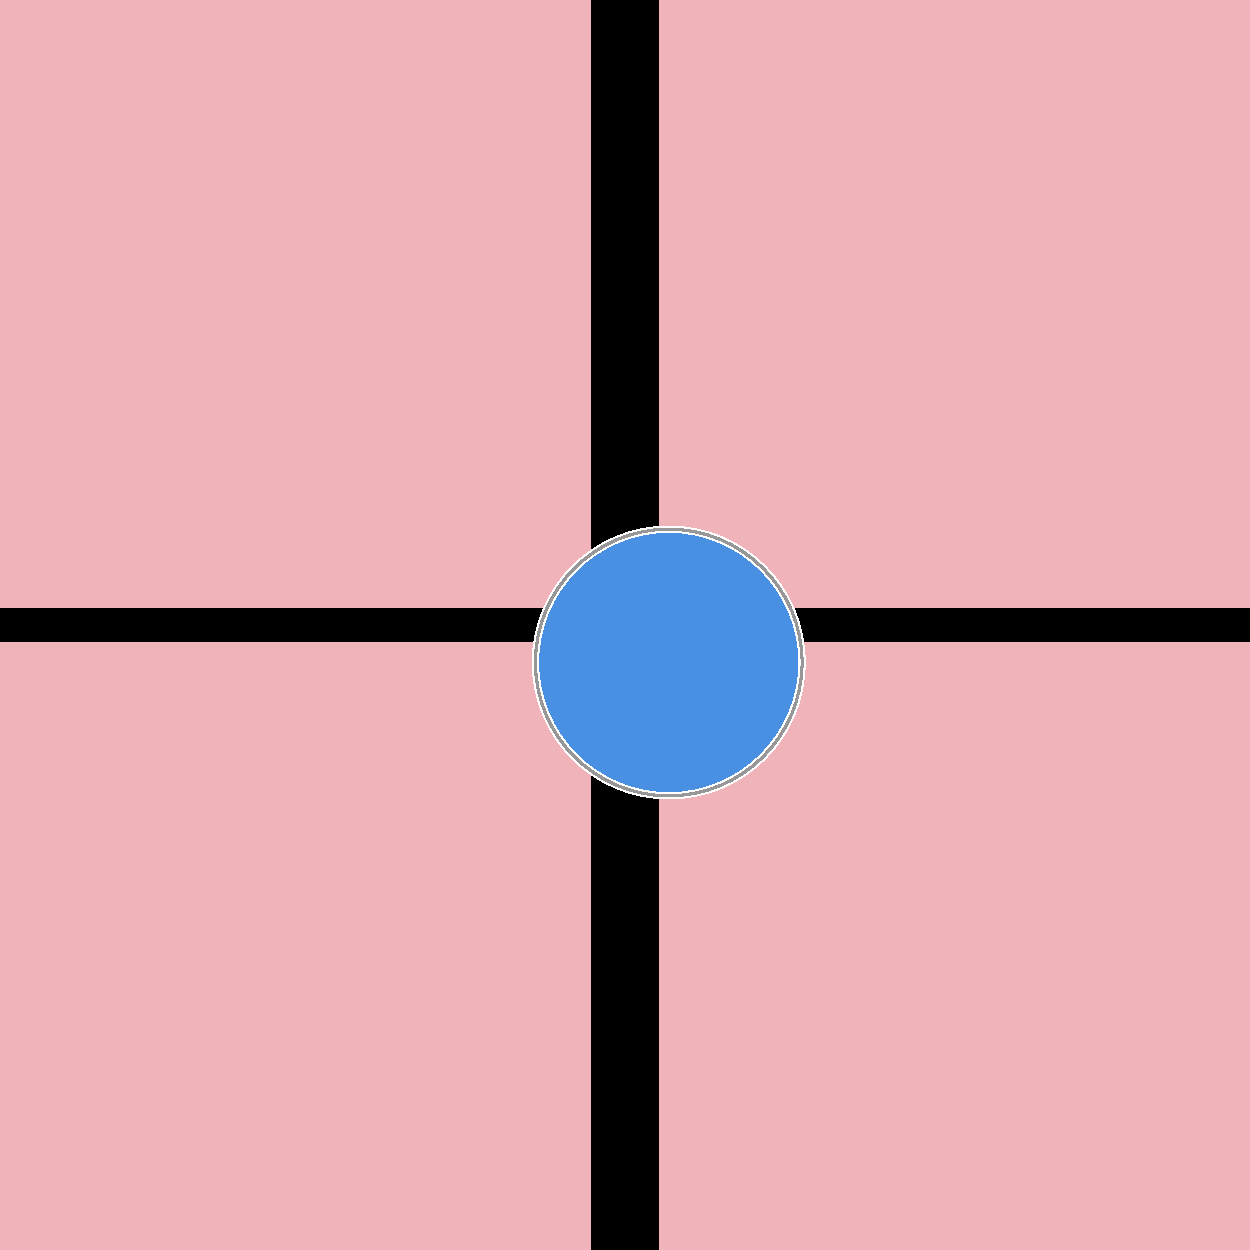
\includegraphics[width=\textwidth]{./resources/worst-case/worst-case-2.pdf}
        \caption{Areas after two splits}
        \label{fig:worst-case:two}
    \end{subfigure}
    \hfill
    \begin{subfigure}[t]{0.11\textwidth}
        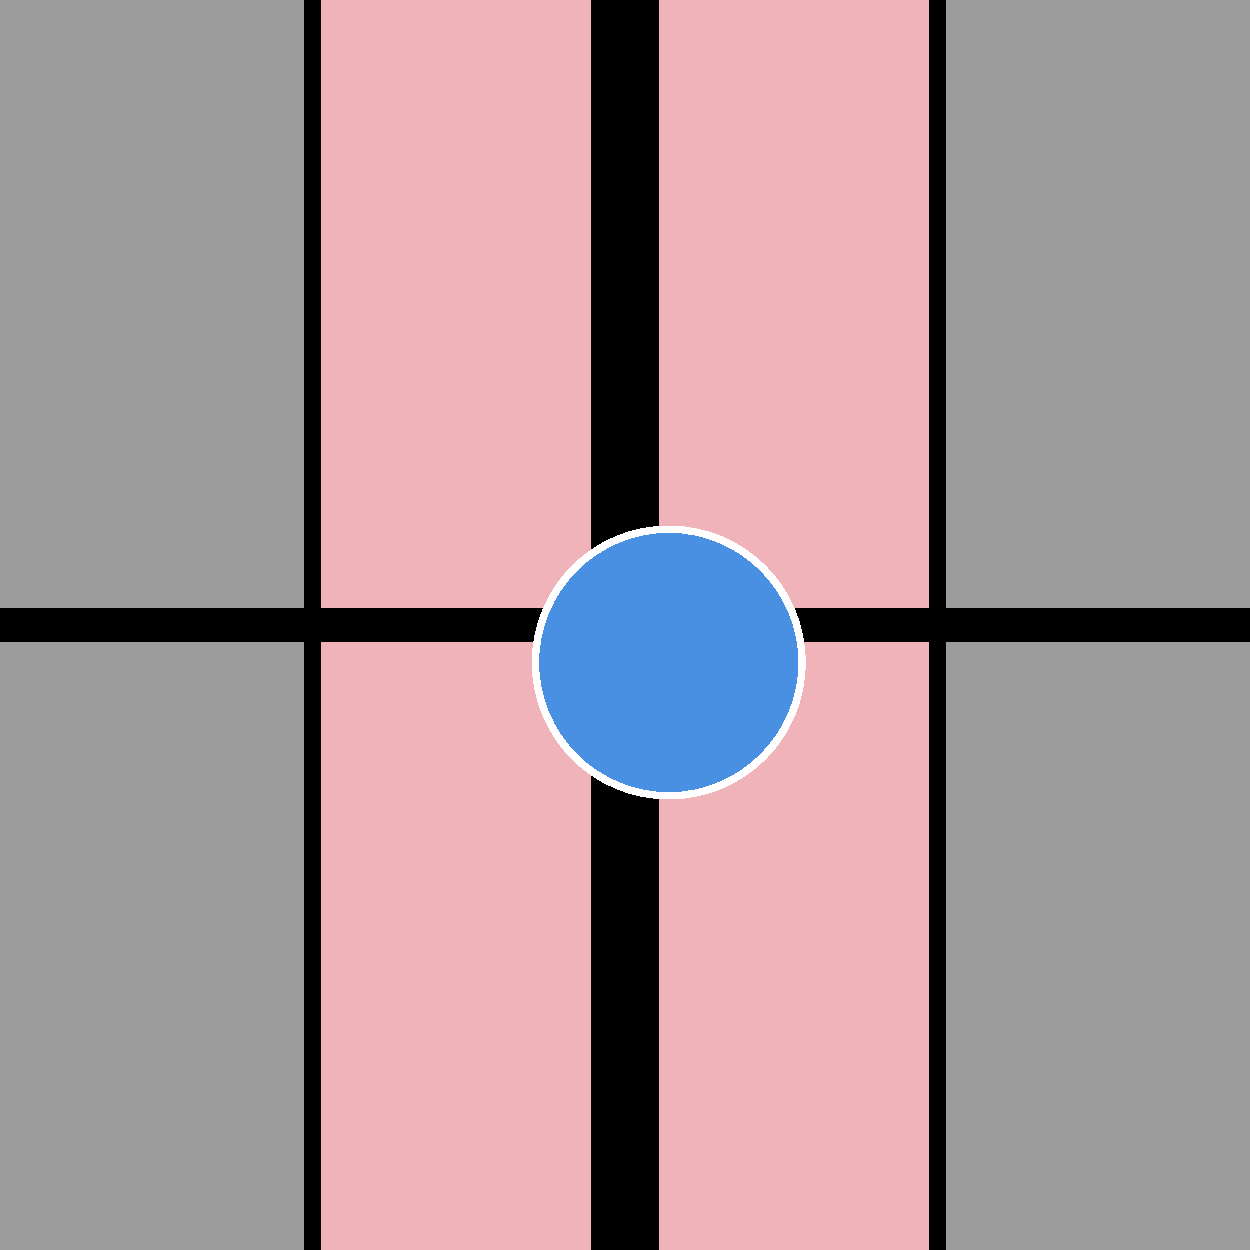
\includegraphics[width=\textwidth]{./resources/worst-case/worst-case-3.pdf}
        \caption{Areas after three splits}
        \label{fig:worst-case:three}
    \end{subfigure}
    \hfill
    \begin{subfigure}[t]{0.11\textwidth}
        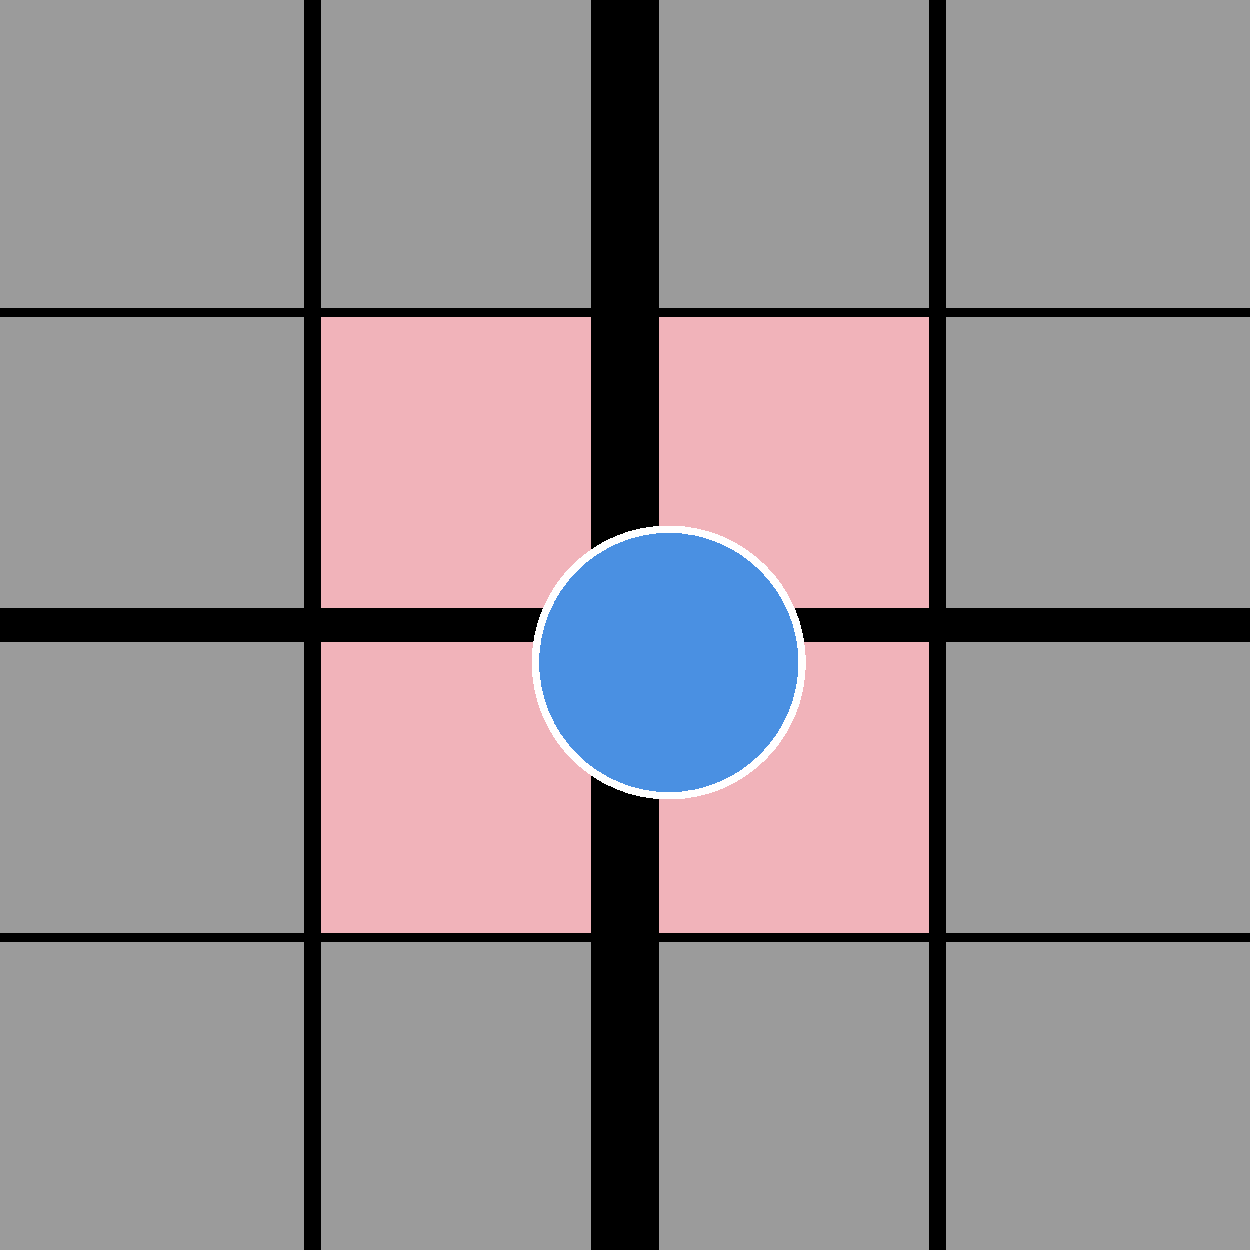
\includegraphics[width=\textwidth]{./resources/worst-case/worst-case-4.pdf}
        \caption{Areas after four splits}
        \label{fig:worst-case:four}
    \end{subfigure}
    \caption{
    	The two-dimensional surface (longitude, latitude) after the first, second, third and fourth split.
    	The blue circle shows a possible area to be claimed by a certificate or the desired query area of a client.
    	The area colored in red is the minimum area that has to be retrieved using the given number of splits.
    }
    \label{fig:worst-case}
\end{figure}

The discretization used by GeoPKI does not directly fit all requirements.
On one hand, claimed volumes will likely never fit exactly one of the voxels.
Moreover, clients likely want to query volumes not aligning with the GeoPKI voxels. 

In both cases this volume $V$ has to be approximated using the GeoPKI voxels.
A trivial approximation the smallest volume encompassing all of $V$.
Unfortunately this results in returning the whole tree if $V$ lies at the intersection of one of the first few division lines.
\Cref{fig:worst-case} depicts this situation with the blue circle corresponding to $V$ and the red area the minimum area that has to be retrieved at the different levels in the tree.
\Cref{fig:worst-case:one} shows the line of the first split.
Given the blue circle intersects both area, the above trivial approximation would result in the whole tree being returned for a comparable small area that is just placed unfortunately.

Thus a better approximation is required.
The main problem with the trivial approximation is the discrepancy of the area queried and the returned area:
If the client queries for a large area, it is fine to return a lot of data.
But in case of a query for a small area, the size of the returned data should be in relation to the queried area.
Given the split lines do not move when going to a deeper level in the tree, it is always necessary to return multiple voxels.
The number of required voxels is monotonically increasing when going deeper down in the tree but the area covered by them monotonically decreases as the voxel approximation for $V$ becomes more accurate.

\subsubsection{Claimed Volumes to Voxels}

In case of the placement of certificates in the tree, it is infeasible to place certificates claiming a volume $V$ in all leaves covered by $V$ due to the loss in sparsity and the resulting explosion in storage requirements.
As noted before, most places on earth are claimed by at least one country and thus the tree would not be sparse at all.

One possible heuristic balancing the returned data size with the number of subtrees loss in sparsity is to use a subtree level where the volume of $V$ is greater than or equal to a given factor $f \in [0, \infty)$ of the voxel volumes at this level.
For instance $f = \frac{1}{4}$ would result in \Cref{fig:worst-case:three} and $f = \frac{1}{2}$ in \Cref{fig:worst-case:four} (assuming all shown areas cover the full altitude spectrum).
% Another heuristic would not use $f$ for the general subtree level volume but for each individual voxel, i.e. only use a specific voxel for a given polyhedron if that polyhedron covers at least the fraction $f$ of the voxel's volume.
The effectiveness of this heuristic and a good value for $f$ is to be determined.

\subsubsection{Query to Voxels}

For the transformation of queries to voxels to be queried the case turns out to be easier.
In terms of response size it is always best to retrieve all individual leaves as directly querying a area higher up in the tree (including it's whole subtree) will always be a superset of that data.

\subsection{Proofs of Presence and Absence}
\label{sec:data-structure:precense-absence}
Given a query for a volume, the map server should prove that the returned data is in fact in the SMT and that no certificate was omitted.
Let $V$ be the set of non-empty voxel that intersect with the query volume and for each $v \in V$ let $\mathcal{C}_v$ be the set of all certificates associated with $v$.
For each such $v \in V$, the server has to send the set $\{H(x) \: | \: \forall x \in \mathcal{C}_v \}$ to the client as it is required to compute the node's hash (see Equations \ref{eq:hash-leaf} and \ref{eq:hash-certs-intermediate-node}).
Due to the fact that parent voxels always cover a super-volume of their children, $V$ includes the transitive closure of the parent relation.
For nodes where a child is not in $V$, this child's hash has to be included in the server's response as it is necessary to compute the node's hash as shown in see Equation \ref{eq:hash-intermediate-node}.

In a sparse SMT, proving the absence of any certificate in a volume is the same as providing the data  within that volume along with a proof which then allows a client to verify its absence.
Similarly, the presence of an empty node proofs the absence of any certificates in that subtree.

Given the binary SMT has $2^{B}$ leaves (see \Cref{sec:data-structure}), it's depth is $B$.
A proof of presence for a node $v$ at depth $d \in \{0, ..., B-1\}$ (zero is the root itself) then consists of the $d$ complementary node's hash along the path to the root.
The size of these hashes is $256$ bits or $32$ bytes due to the use of SHA-256.
Thus in the worst case a proof for a single leaf consists $\left(B-1\right) \cdot 32$~B $= 66 \cdot 32$~B $= 2'112$~B $\approx 2$~KiB and is thus in the same order as an average X.509 certificate.
The size of such a proof is smaller the sparser the tree is and is always smaller if an intermediate node, i.e., not a leaf, is queried.

\subsection{Proof of Consistency}
\label{sec:data-structure:consistency}
As in F-PKI~\cite{chuat_f-pki_2022} using a consistency tree over the root hashes.

\section{Optimization Goals}
\label{sec:optimization-goals}

There are several factors a GeoPKI implementation should optimize for. This includes response size, response latency, the number of requests that can be answered per second (throughput) but also the server storage space and insertion time.
Some of these criteria conflict and some balance between them has to be found.
One example for such a conflict is response size and server storage space which was already mentioned in \Cref{sec:data-structure:arbitrary-volumes}.
Placing certificates higher up in the tree reduces the number of places where the certificate has to be stored but leads to the certificate being included in queries where the query volume does not intersect the certificate's polygon but the voxel it is stored at.
Placing them exclusively in voxels that are fully covered by the polygon and only use full-depth voxels for partially covered ones reduces the likelihood of it being included in a query unnecessarily as far as possible.
Unfortunately this leads to many full-depth voxels (i.e. reduces sparsity / increases the required storage) and increases the response size close to the border of a polygon as a certificate has to be included multiple times, once for each voxel in which it is present.
Moreover the more complex the approach the more complex (and likely slower) the insertion.
The following Sections discuss what the different goals depend on.

\subsection{Response Size}
The response size depends on the number of non-empty voxels intersecting a given query volume.
This in turn depends on the number of certificates in the system, the spatial distribution of their volumes, the query volume and how certificates are assigned to voxels.
Specifically the number of returned superfluous certificates and the number of returned duplicate certificates (when stored in multiple voxels within the query volume) should be minimized.

\subsection{Response Latency and Throughput}
Response latency and throughput depend the response size but also the concrete software implementation and the hardware the implementation is running on.

\subsection{Storage Requirements}
The required storage depends on the total number of certificates in the system, their spatial distribution, how certificates are assigned to voxels but also the concrete software implementation.
For the assignment, reducing the number of voxels where a given certificate is stored should be minimized.

\subsection{Insertion Time}
Insertion time will mostly depend on how certificates are assigned to voxels, the concrete software implementation and the hardware it is running on.
For the certificate assignment, the assignment algorithm's runtime complexity and number of voxels where a given certificate is stored should be minimized.

\subsection{Summary}
Assuming the soft- and hardware are optimized, finding the aforementioned balance between returning superfluous certificates and storing certificates in too many voxels seems to be the factor influencing most optimizations goals.
Having a higher precision than the average query size does not make sense as this can only increase the number of certificates that are returned multiple times because they are assigned to multiple small voxels.
Assuming an average query radius of $r := 10$~m, the precision $u = 2 \cdot r$ intersects at most $2^3 = 8$ leaf voxels, two along each dimension.
In the worst case, all of the dimensions align with the first split in the respective dimension.
For the altitude this would mean that each pair of voxels with the same longitude and latitude bounds share at least $B_x + B_y$ voxels in the hierarchy or rather it is possible to omit $(2^2 - 1) \cdot (B_x + B_y)$ voxel duplicates.
For the longitude and latitude, in the worst case only the two top levels are shared meaning it is only possible to omit the root three times and the two nodes at the second level once.
Thus including the hierarchy, in the worst case $2^3 \cdot B - (2^2 - 1) \cdot (B_x + B_y) - 3 \cdot 1 - 2 = 288$ voxels have to be returned.

In the best case they are all adjacent in the tree, i.e. the path matches until depth $B_x + B_y - 2$ for all of them allowing the omission of seven times that number of voxels.
After this depth, two levels are required for the four distinct longitude/latitude boundaries.
Within each of them, the two leaf voxels can share a path of up to $B_z - 1$ allowing the omission of four times number of voxels.
Thus including the hierarchy, in the best case $2^3 \cdot B - (2^3 - 1) \cdot (B_x + B_y - 2) - 2^2 \cdot (B_z - 1) = 103$ voxels.

%Both of these estimates assume all leaf voxels at the full depth are non-empty which will likely only be the case in cities.
%Assuming the voxel assignment is done more precisely, having sub $20$~m precision reduces the likelihood of fetching redundant certificates whose polygon does not intersect the query sphere but is assigned to the neighboring voxel which does intersect the query sphere.
%The problem is that along the border of a polygon this results in many voxels with the same certificate and the likelihood of a query intersecting not just one but multiple of them increases.
%In this scenario the number of duplicate certificate hashes returned would


\section{Server Implementation}
\label{sec:implementation}

Due to the size of data it seems reasonable to use a data management engine on the server's side, storing the whole data structure in memory is infeasible at the time of writing.

\subsection{Querying for a Sphere Efficiently}
\label{sec:implementation:query-sphere}

\begin{figure}
	\centering
    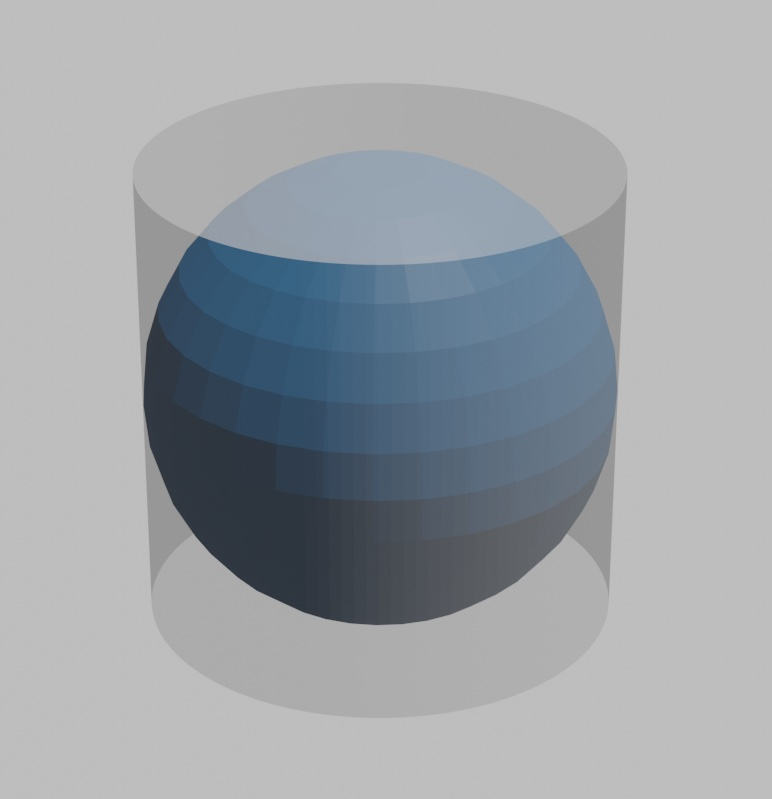
\includegraphics[width=0.25\linewidth]{./resources/query-approximation/cylinder}
    
    \caption{
    	Approximating a sphere using a cylinder.
    }
    \label{fig:sphere-approximation}
\end{figure}

One possibility to query a sphere is to walk the tree and intersect it with the volumes on each level of the tree.
This process is repeated recursively until the reached level is a (sparse) ``leaf''.
When walking the tree like this, all information that has to be returned (including the data for the proof) is obtained in one go.
Such a process would require writing a custom database index which for the moment is out of scope.

\subsubsection{Spatial Index}
Fortunately there are alternatives.
Both, MySQL and PostgreSQL have support for two dimensional geodetic coordinates, PostgreSQL additionally supports three dimensional cartesian coordinates but none of them supports two dimensional geodetic coordinates plus a third cartesian altitude dimension.
Transforming points to earth-centered, earth-fixed (ECEF) cartesian coordinates is straight-forward but the same does not apply to volumes since the coordinate system's grid lines are different.
In the geodetic coordinate systems grid lines are curved while in a cartesian coordinate system they are straight lines.
Hence the shape of volumes defined by their vertices is wildly different and would need to be over-approximated when wanting to use the three dimensional spatial index.
While possible, such over-approximations do not seem trivial to compute. 

Alternatively it is possible to directly make us of the two-dimensional spatial index with support for geodetic coordinates.
In this approach the altitude is initially ignored and the voxel's two dimensional projection to the earth's surface is intersected with a circle with the sphere's radius whose center is the sphere's center also projected to earth's surface.
After querying the spatial index for this, the returned data can be filtered based on the altitude.
Note that this type of query no longer searches for volumes intersecting a sphere but rather over-approximates the sphere as an extruded circle, i.e. a cylinder (see \Cref{fig:sphere-approximation}).
Due to the projection to the earth's surface, the radius of the cylinder has to be adjusted.
When projecting two-dimensional shapes defined by vertices from higher altitudes to the earth's surface (by keeping the longitude and latitude but omitting the altitude), their area shrinks.
Geodetic coordinates simply express the location on the two-dimensional ellipsoid surface where with increasing altitude the corresponding ellipsoid and thus surface area grow.
Analogously when projecting shapes at negative altitudes, their area grows.
This needs to be taken into account when performing the intersection with a circle on earth's surface.
Assuming the original sphere that is queried for is below WGS84's ellipsoid surface and has a radius $r$, the radius used for computing the intersection on earth's surface has to be greater than $r$ since the distance between the sphere's center and all other points on that altitude has increased.
Analogously, the radius can be decreased if the sphere's altitude is above the ellipsoids surface but in this case it is not necessarily required as over-approximating the result is fine when only considering correctness.
Since it is the distances and not areas or volumes that are of interest, the circumferences of ellipses with the different radii should be compared.
Given there is no easy formula for the circumference of an ellipse, the difference is over-approximated by considering spheres instead.
The circumference of an ellipsoid is greater than the circle with a radius corresponding to the length of the ellipse's semi-minor axis ($b$ for WGS84).
Similarly, an ellipsoids circumference is smaller than the circle with a radius corresponding to the length of the ellipse's semi-major axis ($a$ for WGS84).
Thus the fraction by which distances grow from altitude $h$ with $h < 0$ to the earth's surface can be over-approximated as
\begin{align}
\begin{split}
	&\frac{\text{circumference of WGS84 ellipse at }z=0}{\text{circumference of WGS84 ellipse at }z=h}\\
	&\leq \frac{\text{circumference of circle with radius } a}{\text{circumference of circle with radius } (b+h)}\\
	&= \frac{2 a \pi}{2 (b+h) \pi} = \frac{a}{b+h}\\
	&\\
\end{split}
\end{align}

For $h = D$ this results in $\leq 1.005$.

Analogously the fraction by which distances shrink from altitude $h$ with $h > 0$ to the earth's surface can be over-approximated as
\begin{align}
\begin{split}
	&\frac{\text{circumference of WGS84 ellipse at }z=h}{\text{circumference of WGS84 ellipse at }z=0}\\
	&\leq \frac{\text{circumference of circle with radius } (a+h)}{\text{circumference of circle with radius } b}\\
	&= \frac{2 (a+h) \pi}{2 b \pi} = \frac{a+h}{b}\\
	&\\
\end{split}
\end{align}

For $h = H$ this results in $\leq 1.007$.
Given the small numbers and the fact that an over-approximation of the result does not affect correctness, a simple implementation could simply consist of multiplying the radius by $1.005$ to account for possible false negatives.
It is probably advisable to account for this on the client's side to facilitate auditing.
Otherwise a server might claim to not be malicious but return wrong results due to wrong approximations.

A query on the server side

\begin{lstlisting}[language=SQL]
SELECT * FROM nodes
WHERE ST_DWITHIN(
    area,
    query_point,
    query_radius
  ) AND
min_altitude_of_bit_string(bit_string) <= (query_z + query_radius) AND
max_altitude_of_bit_string(bit_string) >= (query_z - query_radius)
\end{lstlisting}

where the functions \texttt{min\_altitude\_of\_bit\_string} and \texttt{max\_altitude\_of\_bit\_string} are respectively defined as follows:
\begin{lstlisting}[language=Python]
# python syntax, ljust = right pad
return int(bit_string[52:].ljust(15, "0"), 2)
\end{lstlisting}

\begin{lstlisting}[language=Python]
# python syntax, ljust = right pad
return int(bit_string[52:].ljust(15, "1"), 2)
\end{lstlisting}

Unfortunately the spatial index used by \texttt{ST\_DWIITHIN} is rather expensive resulting in a lower query throughput than one would hope for.
% TODO refer to measurements

\subsubsection{Prefix Matching}
Smaller bit strings represent larger volumes and in allowing a request for all certificates inside such a volume to be concisely represented by such a bit string.
Since in the definition of the bit strings the altitude bits are simply appended to the interleaved longitude and latitude bits, sending a prefix that covers more in the surface dimension will always cover the full height.
Based on the idea of the previous approach of querying a cylinder, it is possible to additionally send a minimum and maximum altitude with a bit string of length $\leq 52$ (whose geometric representation covers the full height).
The server then returns all voxels whose bit string start with the given query bit string whose geometric representation intersects the given altitude range (several subtrees).
Additionally it must return all voxels whose bit string are a prefix of the given query bit string (the path to the tree root).
Seemingly the DB is not able to process the following statement looking for all prefixes efficiently.
\begin{lstlisting}[language=SQL]
WHERE '0100110...' LIKE bit_string || '%'
\end{lstlisting}

To prevent a full table scan, it can be converted in a set of point queries.
Moreover prefix matching is only supported on strings so an additional \texttt{bit\_string\_txt} column has to be created and indexed.
The full query in SQL can then be written as follows:
\begin{lstlisting}[language=SQL]
SELECT * FROM nodes
WHERE bit_string IN (b'0', b'01', ...)
UNION ALL
SELECT * FROM nodes
WHERE bit_string_txt LIKE '0100110...%' AND
min_altitude_of_bit_string(bit_string) <= (query_z + query_radius) AND
max_altitude_of_bit_string(bit_string) >= (query_z - query_radius)
\end{lstlisting}
By (over-)approximating any volume using bit strings, clients can this way query for any desired cylinder.
In order to approximate a desired query volume, the same algorithm that is used to assign voxels to a certificate can be used, possibly with different parameters.
Note that this approach pushes some work to the client to simplify the server's task.
\subsubsection{Integer Range Queries}
Building on the previous approach, it is possible to transform the prefix matching operation into an integer range query.
Each bit string is interpreted as an integer.
For bit strings longer than $52$ bits only the first $52$ (encoding the longitude and latitude) are taken and for bit strings shorter than $52$, the bits are right padded with zeros up to $52$ bits.
The resulting $52$ bits are then interpreted as a (big endian) integer.
More formally the integers are obtained by calling the function \texttt{to\_surface\_integer(bit\_string, c)} with \texttt{c="0"} where \texttt{to\_surface\_integer} is defined as follows:
\begin{lstlisting}[language=Python]
# python syntax, ljust = right pad
return int(bit_string[:52].ljust(52, c), 2)
\end{lstlisting}
The \texttt{bit\_string\_txt} string column is replaced by a \texttt{bit\_string\_52} bigint column.
The a prefix search for some bit string \texttt{query\_bit\_string} can then be replaced by a range search among the integer representations described above.
The lower and upper bounds $L$ and $R$ are then defined as
\begin{align*}
	L &= \texttt{to\_surface\_integer(query\_bit\_string, "0")}\\
	R &= \texttt{to\_surface\_integer(query\_bit\_string, "1")}
\end{align*}

This allows the SQL query to be written as
\begin{lstlisting}[language=SQL]
SELECT * FROM nodes
WHERE bit_string IN (b'0', b'01', ...)
UNION ALL
SELECT * FROM nodes
WHERE
bit_string_52 >= L AND
bit_string_52 <= R AND
min_altitude_of_bit_string(bit_string) <= (query_z + query_radius) AND
max_altitude_of_bit_string(bit_string) >= (query_z - query_radius)
\end{lstlisting}

The following proof shows this returns all desired results.
Proof by contradiction:
Assume some row that should have been in the results is missing.
The bit string corresponding to the row must be longer than the queried bit string, otherwise it would be a prefix of it and thus explicitly listed in the first part of the query (i.e. \texttt{IN (...)}).
Moreover the row must share all initial bits with the bits with the queried bit string, otherwise it is not supposed to be returned.
Thus its integer value must be between $L$, the minimum value with all zeros after the queried bit string prefix, and $R$, the maximum value with all ones after the queried bit string prefix.

It is left to show that this does not return more results than required but this is not true since additional results are returned.
Interestingly the additionally returned results are a subset of the prefixes that we want to retrieve anyway though so it only reduces the number of prefixes that have to be explicitly listed in the first query part.
More specifically, the query returns all rows whose bit string, the queried bit string is a prefix for plus all prefixes of the queried bit string that can be obtained by omitting trailing zeros.

Proof:
If the queried bit string is a prefix for a row's bit string, it should be returned so assume this is not the case.

\textbf{Case 1:} Assume the corresponding bit string's length is greater than or equal to the queried bit string's.
Since the queried bit string is not a prefix, there must be a position in the query bit string two two bit strings have a different bit.
This results in the corresponding integer representation being strictly greater than $R$ (if it has a $1$ in the position where the query bit string has a $0$) or strictly smaller than $L$ (if it has a $0$ in the position where the query bit string has a $1$).
Thus it violates the condition and cannot be returned by the second part of the query.
Moreover the first part of the query only covers prefixes of the queried bit string which are by definition strictly shorter and thus it also cannot be returned by the first part of the query.
Hence this assumption leads to a contradiction.

\textbf{Case 2:} Assume the corresponding bit string's length is strictly smaller than the queried bit string's.

Assuming the row's bit string is not a prefix of the queried bit string, then by the same argument as in case 1 there must be a position where the two have mismatching bits resulting in the integer bounds being violated.
Moreover it not being a prefix by definition prevents it from being included by the first part of the query.

Hence the last remaining case is when the row is a prefix of the queried bit string.
While in any case this is a row we want, it is possible to narrow down exactly what additional prefixes are returned.
In the best case it would be all of them but unfortunately this is also not the case.
Since integers are zero extended to $52$ bits, the integer representations of two bit strings is the same if they match when omitting all trailing zeros.
And this is exactly the set of additional prefixes that are returned.
Removing a trailing zero does not change the integer representation while removing a trailing one effectively replaces this one with a zero in the integer representation.
Replacing a one with a zero means it the integer does not satisfy the range bounds as it will be too small.

\subsection{Database Tables and Schemas}
\label{sec:implementation:schemas}

When using a integer range query as described in \Cref{sec:implementation:query-sphere}, the tables \texttt{nodes} and \texttt{certificates} are used.
The table \texttt{nodes} has the following columns:
\begin{itemize}
	\item \texttt{bit\_string} of type \texttt{bit varying (66)}
	
	Stores the bit strings described in Sections \ref{sec:data-structure:leaf-binary} and \ref{sec:data-structure:intermediate}.
	There is a non-clustered index on this column enabling fast point queries.
	\item \texttt{bit\_string\_52} of type \texttt{bigint} (64 bit integer)
	
	Stores \texttt{to\_surface\_integer} called on the \texttt{bit\_string} column with \texttt{c="0"} to enable fast range queries.
	There is a B-Tree index on this column and the table is clustered by this index.
	\item \texttt{certificate\_hashes} of type \texttt{bytea[]}
	
	Stores the hashes of the certificates belonging to this node and is by default an empty array.
	The hashes are foreign keys to the \texttt{certificates} table.
	\item \texttt{neighbor\_hash} of type \texttt{bytea | null}
	
	Stores the hash of the node corresponding to the row's neighbor in the SMT (flipping the last bit in the row's bit string) if it is non-empty and otherwise is equal to null.
	This hash might be required for the SMT proof when a row is retrieved.
	\item \texttt{left\_child\_hash} of type \texttt{bytea | null}
	
	Stores the hash of the node corresponding to the row's left child in the SMT (adding a $0$ to the row's bit string) if it is non-empty and otherwise is equal to null.
	This hash might be required for the SMT proof when a row is retrieved.
	\item \texttt{right\_child\_hash} of type \texttt{bytea | null}
	
	Stores the hash of the node corresponding to the row's right child in the SMT (adding a $1$ to the row's bit string) if it is non-empty and otherwise is equal to null.
	This hash might be required for the SMT proof when a row is retrieved.
\end{itemize}

All columns other than \texttt{bit\_string} and \texttt{certificate\_hashes}, are redundant and could be computed based on other information inside the database but are stored explicitly to speed up queries.
To ensure consistency, constraints are used.

The \texttt{certificates} table only consists of two columns, the primary key \texttt{certificate\_hash} of type \texttt{bytea} storing the SHA256 hash of the certificate and the column \texttt{certificate}, also of type \texttt{bytea}, storing the certificate itself.

\section{Alternative Designs}
\label{sec:alternative-designs}

An alternative design could use a (hybrid-)quadtree or (hybrid-)octree where most intermediate nodes have four or eight children, respectively.
For simplicity let's assume $B_{y} = B_{x} = 26 := B_{x,y}$ in the following analysis.
``Hybrid'' and ``most'' because $B_{x} = B_{y} > B_{z}$ which means the volume cannot be subdivided fully using a quad- or octree.
Hence when using an octree with eight children, the $z$ dimension is already exhausted after $B_{z}$ splits and will from there continue to only have four children (i.e. a quadtree).
When using a quadtree, the first $B_{x,y}$ splits would solely concern the $x$ and $y$ dimensions and after that the children will be binary trees of height $B_{z}$ only splitting the $z$ dimension.
This will decrease the tree's height but increase the proof size due to the larger number of neighboring hashes that have to be provided on each level.
For the hybrid-quadtree, the tree height would be $\log_4(2^{2 \cdot B_{x,y}})= \log_4(4^{B_{x,y}}) = B_{x,y} = 26$ plus the $\log_2(2^{B_z}) = B_z = 15$ for the binary subtrees.
For the hybrid-octree the tree height would be
$\log_8(2^{3 \cdot B_z}) = \log_8(8^{B_z}) = B_z = 15$ plus the $\lceil \log_4(2^{B - 3 \cdot B_z}) \rceil = 21$ for the quad-subtrees.
The proof size of a leaf would thus increase to $(26 \cdot (4 - 1) + (15 - 1) \cdot (2 - 1)) \cdot 32$~B $= 2'944$~B $\approx$ $3$~KiB and $(15 \cdot (8 - 1) + (21 - 1) \cdot (4 - 1)) \cdot 32$~B $= 3'630$~B $\approx$ $3.5$~KiB, respectively.
The ones are subtracted from the tree height since the on the last level no complementary hash has to be returned.
The ones subtracted from the number of neighbors is due to the fact that the hash resulting from the leaf itself does not have to be provided as it can be computed by the client.

Unfortunately the worst case scenario remains:
Two spatially adjacent volumes intersecting the lines of the first split only share the root node as a common ancestor.
When using a tree this will always be the case due to nodes having a single parent.
Consider single dimensional discrete consecutive numbers and a binary tree.
Each number (except the start and end) has two numerically neighbors but can only have one neighbor in the tree.
This fact also holds for group of leaves and thus there will always be two numerically close neighbors just sharing the root node as their ancestor.

To maintain consistency with the already introduced binary representation of volumes, one can consider the quad-tree part (i.e. the first $B_{x,y}$ levels) to add two bits to the prefix on each level rather than just one.
The last $B_z$ levels would then each just add a single bit as before.

Since it is not yet clear if and to what extent the usage a more complex tree structure could be beneficial and hence the more simple binary tree is preferred for the moment.

\section{Caveats}
\label{sec:caveats}

Since longitude ($x$) and latitude ($y$) coordinates that are split in half numerically represent polar coordinates on a sphere, numerically equidistant points, areas or volumes are not equidistant on earth.
Near the poles the longitudinal circumference is smaller but represented using the same numerically range resulting in higher precision.
Hence the discretization range was chosen based on the semi-major axis at the equator where the achieved precision is smallest.

\section{Certificate Format}
\label{sec:certificate-format}

The claimed volume has to be specified in the X.509 certificate.
The used format should be flexible enough to support a variety of use cases such as a set of disjoint volumes, rectangular but also circular volumes.
Open Street Maps uses polygons and RFC 7946 specifies the ``geospatial data interchange format'' GeoJSON \cite{butler_geojson_2016} that also makes use of polygons.
One option would be to define additional types allowing for three dimensional polygons, another to use the ``properties'' field defined in RFC 7946.
When going with the latter approach, each certificate could define a \texttt{GeometryCollection} of \texttt{Polygon}s or \texttt{MultiPolygon}s, each with an \texttt{altitude\_from} and \texttt{altitude\_to} property indicating the inclusive minimum and maximum altitude, respectively.
Note that this representation only allows for extruded two dimensional polygons as primitives but their composition allows more complex shapes.
Since the GeoJSON uses a text-encoding, serializing the data using e.g. protocol buffers as done by Mapbox \cite{mapbox_geobuf_2023} will result in a smaller encoding and fast read and write operations.

\bibliographystyle{IEEEtran}
\bibliography{GeoPKI.bib}
\end{document}
